
%% CLASS MANUAL FOUND IN http://blog.poormansmath.net/latex-class-for-lecture-notes/ %%
%% CLASS AUTHOR Stefano Maggiolo %%
\documentclass[english,course]{Notes}

\title{MATHEMATICS 1S}
\subject{Mathematics}
\author{Joao Almeida-Domingues}
\email{2334590D@student.gla.ac.uk}
\speaker{Sergio Giron}
\date{10}{01}{2019}
\dateend{24}{05}{2019}
\place{University of Glasgow}

 %%%%% GENERAL MATHEMATICAL NOTATION SHORTCUTS %%%%%
 
\newcommand{\n}{\mathbb{N}}
\newcommand{\z}{\mathbb{Z}}
\newcommand{\q}{\mathbb{Q}}
\newcommand{\cx}{\mathbb{C}}
\newcommand{\real}{\mathbb{R}}
\newcommand{\field}{\mathbb{F}}
\newcommand{\ita}[1]{\textit{#1}}
\newcommand{\oneton}{\{1,2,3,...,n\}}
\newcommand\ef{\ita{f} }
\newcommand\inv[1]{#1^{-1}}
\newcommand\setb[1]{\{#1\}}
\newcommand\en{\ita{n }}
%\renewcommand\qedsymbol{QED} %QED instead of square

%%%%%%%%%%%%%%%%PACKAGES%%%%%%%%%%%%%%%%%%%%%%%%%%%%%
%\usepackage{lipsum}  

\usepackage{amsmath,amsthm,amssymb,graphicx,mathtools,tikz,pgfplots} %maths
\usepackage{hyperref,framed,color,fancybox} %layout
\pgfplotsset{compat=1.16}

% framed :  \begin{shaded,frame,snugshade or leftbar} \definecolor{shadecolor}{rgb}{XYZ} to change color
%fancybox: \shadowbox,ovalbox or doublebox
%\extra for Extra content layout box
%%%%%%%%%%%%%%%%%%%%%%%%%%%

%%%CLASS SHORTCUTS%%%%
%\lecture{day}{month}{year} for margin note 
%\begin{theorem} sdfsdf\end{theorem}  --> \theorem
%\begin{proposition} dfsdfs\end{proposition} --> \prop
%\begin{lemma} dsfsd \end{lemma} --> \lem
%\begin{corollary} f ffew \end{corollary}
%\begin{definition} fwewef w \end{definition} --> \defn
%\begin{example} feww e\end{example} --> \ex
%\begin{exercise} wefwe \end{exercise}
%\begin{remark} wef we \end{remark} --> \rem
%\begin{fact} wefe \end{fact}
%\begin{problem} wef ew \end{problem}
%\begin{conjecture} ewfew \end{conjecture}
%\begin{claim} few w \end{claim}
%\begin{notation} fewf \end{notation} --> \nota
%\mymarginpar for scriptsize margin

\begin{document}
\newpage

\section{Taylor \& McLaurin Series}

\lecture{10}{01}{2019}
\textbf{Motivation:} Some functions cannot always be easily evaluated (e.g. $\cos(47)$), polynomial functions on the other hand are, one plugs the values in, and after performing some arithmetic  gets an output. Taylor series \ref{taylor:taylordef} are a \textbf{tool for approximating functions, by converting them into polynomials} .\footnote{https://media.giphy.com/media/zZYEX0w4bj8hG/giphy.gif} \\

\noindent\textbf{Geometric Interpretation}
\par{We cannot however choose any polynomial, it must be one which closely resembles the original function. Our first question should then be "When are two functions equal?". Obviously, two functions are equal if they have all points in common, or to put it another way, if they have the same shape. It follows then, that two functions will be \ita{approximately} equal if their shapes match \ita{approximately}.} \\

\par{ Let $f(x) = \cos(x)$ , be the function which we want to approximate near $x = 0$. Let $g(x) = c_0 + c_1x^1 + c_2x^2 + c_3x^2 + \dots $ be a general polynomial.} \\ As it stands we seem to have two different problems (1) We'll need to find the constant terms which make $g(x)$ have a similar shape to that of $f(x)$. (2) We must find a way to obtain a value of the sum, which is not possible for an infinite polynomial.

\begin{enumerate}
	\item Since we know how to evaluate $sin(0) = 0$ , we know that : 
	$$g(0) = 0 \iff g(0) = c_0 + c_1(0)^1 + c_2(0)^2 + c_3(0)^2 + \dots$$ 
	But since any higher order terms \ita(h.o.t) will all be 0 , we find that $c_0 = 0$
	
	At this stage we have the following:


\begin{figure}[h]
\centering
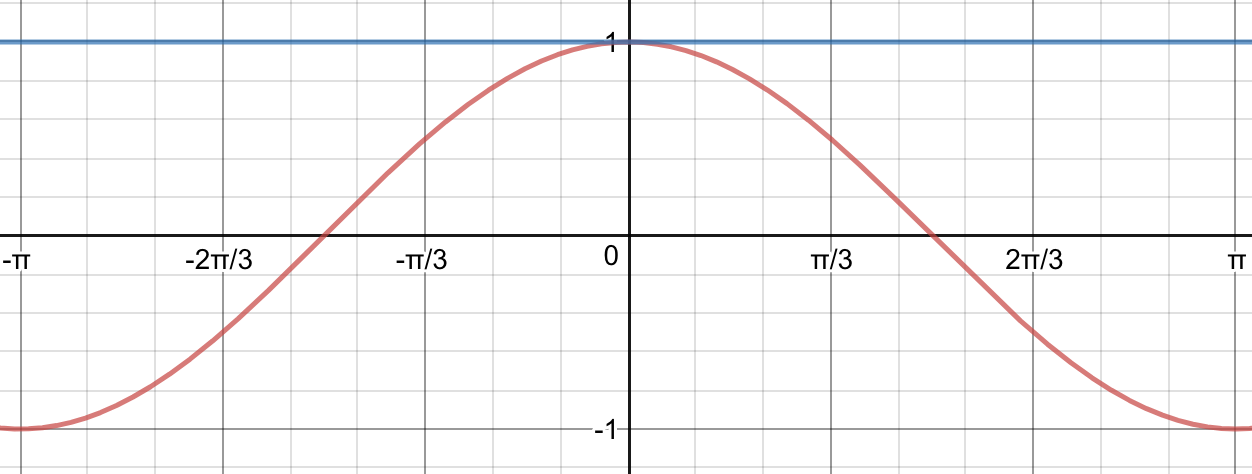
\includegraphics[width=0.5\textwidth]{taylor1st}
\end{figure}


\par{ This is far from a good approximation, but we have found one constant for our polynomial. Next we can think of other information we can get from $cos(x)$ near $x=0$. We know how to differentiate, hence he can get the rate of change of the function at $0$}

\item Finding the first order derivative for $f(x) \text{ and } g(x)$ we have that $f'(0) = -\sin(0) = 0$ and $g'(0) =  c_1 + 2c_2(0) + 3c_3(0)^2 + \dots = c_1$ . Again by equating the two derivatives we find that $c_1 = 0$. We now have: 

$$ g(x) = 1 + c_2x^2 + \cdots $$

\par{ Which did not help much, but we can still get more information, this time from the first-order derivative, and by repeating this process we'll get more and more terms for $g(x)$,and our approximation will be more and more accurate}

\item For up to the $6^{th}$ higher-order derivative we have that :

\begin{figure}[h]
\centering
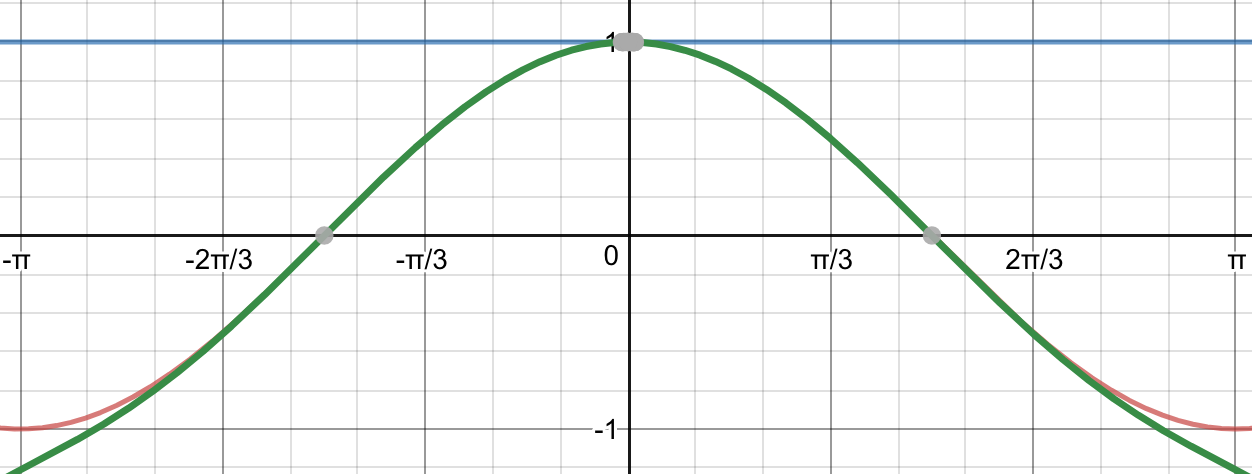
\includegraphics[width=0.5\textwidth]{taylor2nd}
\end{figure}


$$ g(x) = 1 + \frac{x^2}{2} + \frac{x^4}{24} + \frac{x^6}{720} $$

If we plugin a value into our polynomial, we find that the result is $\approx 98\%$ accurate comparing to the one obtained by a calculator. 

We still do not know "when to stop". For a periodic function like $\cos(x)$ this is sort of irrelevant, but for other functions which do not behave so regularly we can erroneously assume that our approximation is accurate anywhere in their domain, which in certain cases would be wrong \ref{taylor:rangeval}. How can we solve our \ita{infinite sum problem}

\item \label{taylor:cN}Lets first note that for each new term we generate, there seems to emerge a pattern. Every time we found a new higher order derivative , every other term we are not considering, remains unchanged *. \mymarginpar{*since they either differentiate to $0$ (l.o.t) or are multiplied by $0$ (h.o.t).} Furthermore, since $g(x)$ is a polynomial, every time we differentiate to find $c_n$ we find that the powers of \ita{h.o.t} accumulate, s.t. when we reach the $n^{th}$ term, the coefficient of $x$ is equal to n! which needs to be cancelled in order to obtain $c_n$, so the inverse is taken. So, at x = 0:

$$ c_n = \frac{1}{n!}f^{(n)}(0) $$

\nota{ $f'^{(n)}$: the $n^{th}$ order derivative}

\item \mymarginpar{*for example, the $18^{th}$ term of our example above yields 0.0000000002679245561}After coming to the conclusion above (\ref{taylor:cN}), we observe that if the series converges \ref{taylor:ratio} towards a limit, then as the \ita{h.o.t} become larger, they become less and less significant*. Let the first $n$ "significant" terms of the polynomial represent a \ita{truncated power series} \ref{taylor:powerSeries} \ref{taylor:taylorpoly} , and all higher order ones - $O(x^{n+1})$ - or - $R_n(x)$ - be the \ita{remainder} of the series. Then if $ \lim_{n\to\infty}R_n(x) = 0$ , $f(x)$is just the sum of the series up until n.

\nota{$O(x^n)$ : All all the omitted terms are of $n^{th}$ order or higher in $x$}

\newpage
\textbf{Putting it all together:}

\defn{Power Series\label{taylor:powerSeries} \ \ \ \ \ }{$ \sum _ { n = 0 } ^ { \infty } a _ { n } x ^ { n }$}

\defn{Taylor Series*\mymarginpar{*of $f$ at $a$}}{$$ \ \ \ \ \sum_{n=0}^{\infty}\frac{f^{(n)}(a)}{n!}(x-a)^n$$ \label{taylor:taylordef}}

\defn{Taylor Polynomial \label{taylor:taylorpoly}}{ A polynomial which higher order derivatives are designed to matchup with the original function (truncated Taylor series}

\rem{Note that the example above evaluates the derivatives at $0$ because it is "cleaner" to do so, but we can start at any point where the value of the function is known. When starting at $0$ the series are called \textbf{McLaurin Series} \ref{taylor:mc} }

\defn{McLaurin Series \label{taylor:mc}}{$$ \ \ \ \ \sum_{n=0}^{\infty}\frac{f^{(n)}(0)}{n!}(x)^n$$}

\defn{Range of Validity\label{taylor:rangeval}}{ The values of $x$ for which the infinite sum exists and is equal to $f(x)$} \mymarginpar{TO DO: Method for finding it}
 
\end{enumerate}

 \extra{The Ratio Test \label{taylor:ratio} \begin{enumerate}
\item Convergent if $\lim_{n\to\infty} = \Big|\frac{a_{n+1}}{a_n}\Big| < 1$
\item Divergent if $ \lim_{n\to\infty} = \Big|\frac{a_{n+1}}{a_n}\Big| > 1$
\item Inconclusive if $ \lim_{n\to\infty} = \Big|\frac{a_{n+1}}{a_n}\Big| = 1$
\end{enumerate}}

\end{document}

